\documentclass[graybox]{svmult}

% |-------------------------------------------------------------------------------------
% | Packages.
% |

% |--------------------|
% | Template Packages
% |

\usepackage{bibentry}
\usepackage{type1cm}           % Activate if the above 3 fonts are not available on your system.

\usepackage{makeidx}           % Allows index generation.
\usepackage{graphicx}          % Standard LaTeX graphics tool when including figure files.

\usepackage{multicol}          % Used for the two-column index.
\usepackage[bottom]{footmisc}  % Places footnotes at page bottom.

\usepackage{newtxtext}
\usepackage{newtxmath}         % Selects TimesNewRoman as basic font.
\usepackage{dirtytalk} \newcommand{\mysay}[1]{\say{\textit{#1}}}
\usepackage{enumerate}
\usepackage[unicode,colorlinks=true,breaklinks,allcolors=black]{hyperref}
\usepackage{cleveref}
\usepackage{ltablex}
\usepackage{booktabs}
\usepackage{hyphenat}
\usepackage{makecell}
\usepackage{doi}
\usepackage{enumitem}

\usepackage{pgfplots}
\pgfplotsset{compat=1.17}
\usepgfplotslibrary{statistics}
\usetikzlibrary{pgfplots.statistics}

\usepackage{fixme}
\usepackage{fancyhdr}

% |--------------------|
% | Personal Packages
% |

% Pozwala na używanie kodu w papierze. // Marcel Jerzyk
\usepackage{listings}

% |--------------------|
% | Personal Definitions
% |

% Creates \code for single-word code highlights // Marcel Jerzyk
\def\code#1{\texttt{#1}}

% Defining new colors for code highlighting
\definecolor{codestring}{rgb}{0.7, 0.3, 0.0}
\definecolor{codegray}{rgb}{0.5, 0.5, 0.5}
\definecolor{codecomment}{rgb}{0.3, 0.4, 0.1}
\definecolor{codekeyword}{rgb}{0.3, 0.8, 0.4}
\definecolor{backcolour}{rgb}{0.95, 0.95, 0.92}

% Creating new language for the Scopus Query highlighting // Marcel Jerzyk
\lstdefinelanguage{Query}{
    backgroundcolor=\color{backcolour},
    keywords={AND, OR},
    keepspaces=true,
    sensitive=true,
    stringstyle=\color{codestring},
    basicstyle=\ttfamily\footnotesize,
    morestring=[b]"
}

% Creating new language for the Python output highlighting // Marcel Jerzyk
\lstdefinelanguage{PythonOwn}{
    backgroundcolor=\color{backcolour},
    basicstyle=\ttfamily\footnotesize,
    keywords={str, int, float},
    keywordstyle={\color{codekeyword}},
    keepspaces=true,
    sensitive=true,
    commentstyle=\color{codecomment},
    stringstyle=\color{codestring},
    comment=[l]{#}, % Err Info: This line provokes an error, the reason why is unknown though
    morestring=[b]"
}

% Creating new language for the script launching highlighting // Marcel Jerzyk
\lstdefinelanguage{BashOwn}{
    backgroundcolor=\color{backcolour},
    keepspaces=true,
    sensitive=true,
    stringstyle=\color{codestring},
    basicstyle=\ttfamily\footnotesize,
%    morestring=[b]'
}


%\nobibliography
\usepackage{fixme}

\nobibliography*


% see the list of further useful packages
% in the Reference Guide

\makeindex             % used for the subject index
                       % please use the style svind.ist with
                       % your makeindex program

% |-------------------------------------------------------------------------------------

\pagestyle{fancy}
\fancypagestyle{firstpage}{
  % Clears the default for header and footer
  \fancyhf{}
  \lhead{\footnotesize Sprawozdanie wykonane przez Marcel Jerzyk, Jakub Litkowski oraz Jakub Szańca dla grupy \code{M2}.}
}
\setlength{\headheight}{110pt}

%%%%%%%%%%%%%%%%%%%%%%%%%%%%%%%%%%%%%%%%%%%%%%%%%%%%%%%%%%%%%%%%%%%%%%%%%%%%%%%%%%%%%%%%%



\begin{document}

\title*{Sprawozdanie z Milestone'u \#2 Grupy M2}
\author{Marcel Jerzyk, Jakub Litkowski, Jakub Szańca}
\institute{
Marcel Jerzyk \at Wroclaw University of Science and Technology, Poland, \email{244979@student.pwr.edu.pl}
\and Jakub Litkowski \at Wroclaw University of Science and Technology, Poland, \email{242353@student.pwr.edu.pl}
\and Jakub Szańca \at Wroclaw University of Science and Technology, Poland, \email{242519@student.pwr.edu.pl}
}

\maketitle

\thispagestyle{firstpage}

\newpage

\section{Performance Test}

Dla każdej próby testu użyto $30\%$ wielkości zbioru uczącego.
Przedstawiemy tabele informacji [\ref{tab:timer}] z czasu wykonywania programu przy pomocy komendy z \code{README.md}:

\begin{lstlisting}[language=BashOwn, label={lst:komenda}]
mvn exec:java -Dexec.args=30
\end{lstlisting}


\begin{table}[!h]
\centering
        
\begin{tabular}{|p{0.33\textwidth}|p{0.33\textwidth}|p{0.33\textwidth}|}
\hline 
 \begin{center}
\textbf{Komputer}
\end{center}
 & \begin{center}
\textbf{Próba}
\end{center}
 & \begin{center}
\textbf{Czas}
\end{center}
 \\
\hline 
 \multirow{$\displaystyle k_{1}$} & $\displaystyle 1$ & 0:01 \\
\cline{2-3} 
   & $\displaystyle 2$ & 0:01 \\
\cline{2-3} 
   & $\displaystyle 3$ & 0:01 \\
\hline 
 \multirow{$\displaystyle k_{2}$} & $\displaystyle 1$ & 4:12 \\
\cline{2-3} 
   & $\displaystyle 2$ & 4:15 \\
\cline{2-3} 
   & $\displaystyle 3$ & 4:11 \\
\hline 
 \multirow{$\displaystyle k_{3}$} & $\displaystyle 1$  & 7:47 \\
\cline{2-3} 
   & $\displaystyle 2$ & 7:51 \\
\cline{2-3} 
   & $\displaystyle 3$  & 7:37 \\
 \hline
\end{tabular}
\label{tab:timer}
\end{table}

oraz w tabeli \ref{tab:timer2} dla komendy:

\begin{lstlisting}[language=BashOwn, label={lst:komenda}]
mvn exec:java -c
\end{lstlisting}

\begin{table}[!h]
\centering
        
\begin{tabular}{|p{0.33\textwidth}|p{0.33\textwidth}|p{0.33\textwidth}|}
\hline 
 \begin{center}
\textbf{Komputer}
\end{center}
 & \begin{center}
\textbf{Próba}
\end{center}
 & \begin{center}
\textbf{Czas}
\end{center}
 \\
\hline 
 \multirow{$\displaystyle k_{1}$} & $\displaystyle 1$ & 13:23 \\
\cline{2-3} 
   & $\displaystyle 2$ & 12:54 \\
\cline{2-3} 
   & $\displaystyle 3$ & 13:11 \\
\hline 
\end{tabular}
\label{tab:timer2}
\end{table}


Przy czym konfiguracja komputerów $k_{1}, k_{2}, k_{3}$ jest następująca:

\begin{table}[!h]
\centering
        
\begin{tabular}{|p{0.20\textwidth}|p{0.20\textwidth}|p{0.20\textwidth}|p{0.20\textwidth}|p{0.20\textwidth}|}
\hline 
 \begin{center}
\textbf{Komputer}
\end{center}
 & \begin{center}
\textbf{CPU}
\end{center}
 & \begin{center}
\textbf{GPU}
\end{center}
 & \begin{center}
\textbf{OS}
\end{center}
 & \begin{center}
\textbf{RAM}
\end{center}
 \\
\hline 
 $\displaystyle k_{1}$ & Ryzen 3600 & RTX 2060 2GB & Windows 10 & 32GB @ 1600MHz \\
\hline 
 $\displaystyle k_{2}$ & Intel Core i5  3340M & Intel HD Graphics & Linux Debian 10 & 4GB @ 1600 MHz \\
\hline 
 $\displaystyle k_{3}$ &Intel Core i5-7200U  &Intel HD Graphics 620  & Windows 10 & 12GB @ 2133MHz  \\
 \hline
\end{tabular}
\end{table}

\begin{figure}[!h]
\centering
\includegraphics[width=\linewidth]{img/report_for_m2/m2_2_report_1.png}
\end{figure}

\begin{figure}[!h]
\centering
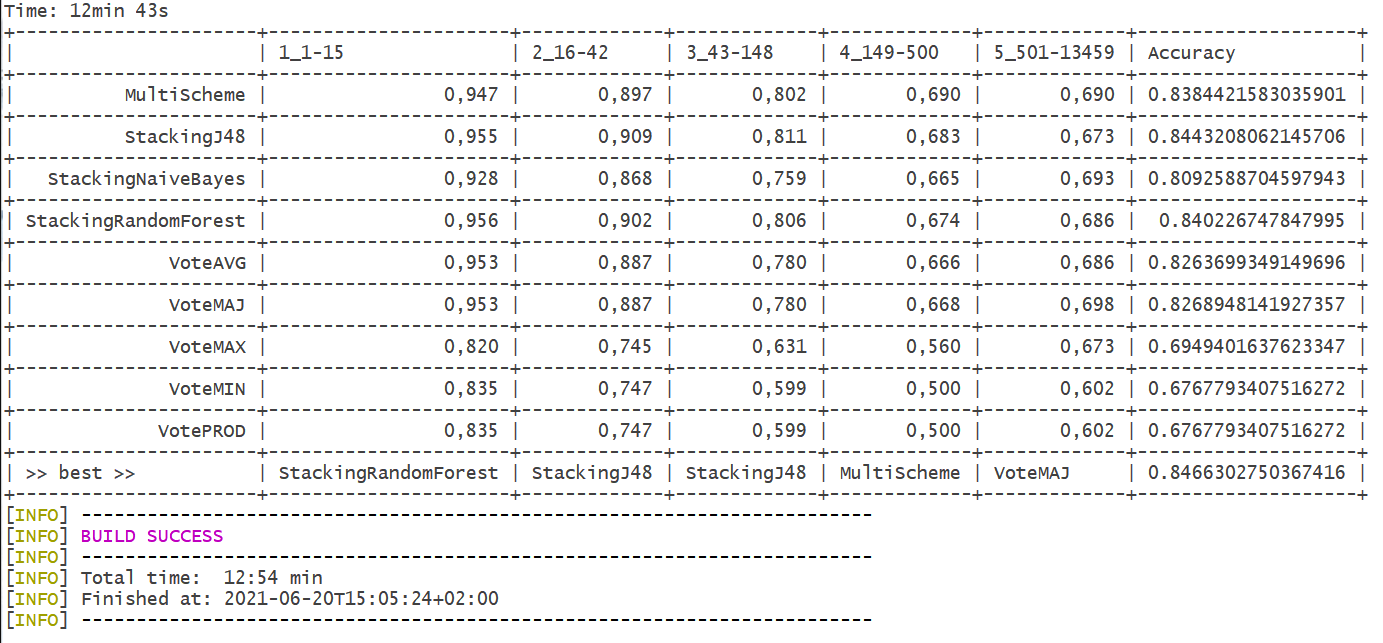
\includegraphics[width=\linewidth]{img/report_for_m2/m2_2_report_2.png}
\end{figure}


\clearpage

\section{Uwagi}

\subsection{Plik objaśniający}
Plik \code{README.md} na głównym branchu wciąż wskazuję na branch odnoszący się do reprodukcji pierwszego milestone. W związku z tym trudno jest odnaleźć instrukcje reprodukcji badań dotyczącą drugiego milestone. Instrukcja jest zwięzła, posiada informacje na temat wykonywanych badań. Występuje informacja o badanych meta klasyfikatorach w wynikach programu. Nie ma informacji na temat użytych bibliotek i ich wersji.

\subsection{Kod}

Kod aplikacji jest odpowiednio podzielony na pakiety oraz ogólnie przejrzysty. Występuje bardzo duża ilość zduplikowanych linii oraz tokenów w języku \emph{R} - blisko aż $50\%$ w obu przypadkach, natomiast kod w \emph{Javie} jest napisany bardzo dokładnie i z pomyślunkiem - w nim nie wystąpiły żadne duplikaty.

\begin{figure}[h]
\centering
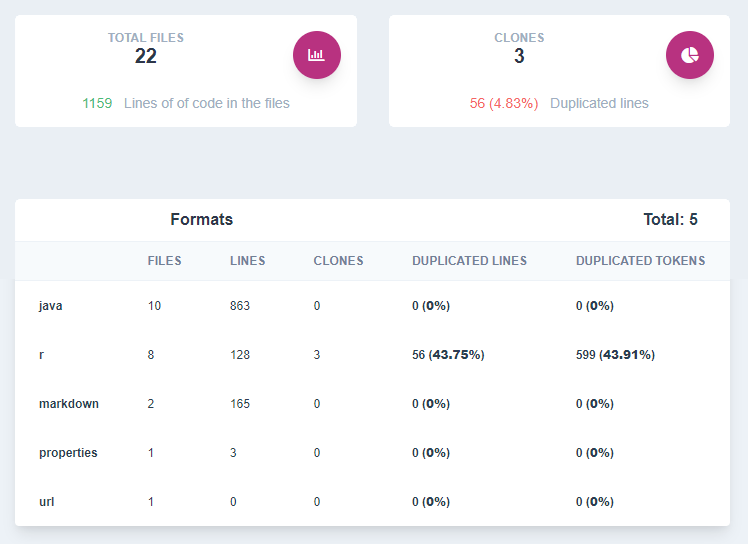
\includegraphics[width=\linewidth]{img/report_for_m2/m2_2_static_analysis.png}
\end{figure}

Z kolei za to, wykryto $224$ błędów w \emph{Javie} przy pomocy lintera \emph{Checkstyle} \footnote{Strona \emph{Checkstyle} - \url{https://checkstyle.sourceforge.io/}}, z czego:

\begin{itemize}
  \item $70$ \code{[LineLength]}: \\ Errory spowodowane zbyt długą ilością znaków w linii (powyżej $80$) 
  \item $23$ \code{[JavadocVariable]}: \\ Errory związane z brakiem dokumentacji zmiennych 
  \item $25$ \code{[MissingJavadocMethod]}: \\ Errory związane z brakiem dokumentacji metod 
  \item $13$ \code{[MagicNumber]}: \\ Tzw. ,,magiczne cyfry'' 
  \item $72$ \code{[FinalParameters]}: \\ Parametry, które mogłyby mieć label \code{final} 
  \item $1$ \code{[AvoidStarImport]}: \\ Sugestia nieużywania importu z gwiazdką 
  \item $10$ \code{[DesignForExtension]}: \\ Bad Smell dotyczący designu klasy, który wygląda jakby miała być reużywalną, ale nie ma \emph{javadoc}, badź \emph{final}, czy też innych annotacji 
  \item $2$ \code{[WhitespaceAround]}: \\ Brakująca spacja przed / po znakach matematycznych.
  \item $5$ \code{[HideUtilityClassConstructor]}: \\ Klasy ,,użytkowe'' nie powinny mieć publicznych, bądź domyślnych konstruktorów
  \item $1$ \code{[ModifierOrder]}
  \item $3$ \code{[HiddenField]}
\end{itemize}

Nastomiast dla \emph{R} wykryto $68$ błędów stylistycznych oraz $4$ warningi, przy pomocy lintera \emph{lintr} \footnote{Strona domowa \emph{lintr} - \url{https://cran.r-project.org/web/packages/lintr/index.html}}.

\begin{figure}[h]
\centering
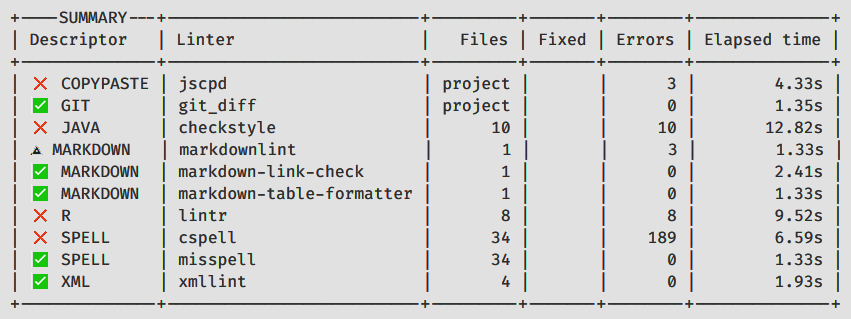
\includegraphics[width=\linewidth]{img/report_for_m2/m2_2_errors.png}
\end{figure}

\clearpage

\subsection{Report}

Prezentujemy zaimportowane dane z wygenerowanego raportu w programie Excel. \\


\begin{figure}[!h]
\centering
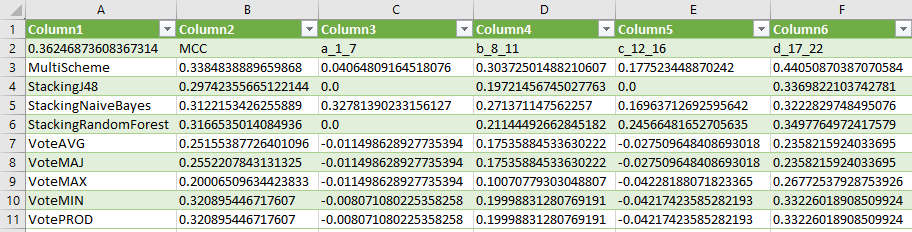
\includegraphics[width=\linewidth]{img/report_for_m2/m2_2_results_1.png}
\end{figure}

\begin{figure}[!h]
\centering
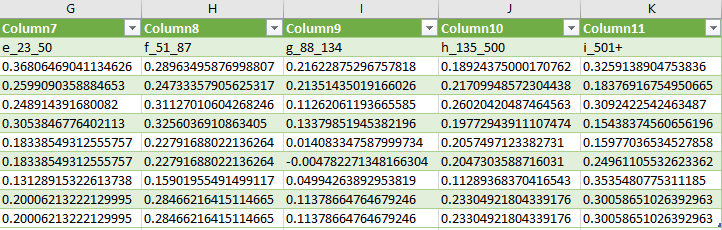
\includegraphics[width=\linewidth]{img/report_for_m2/m2_2_results_2.png}
\end{figure}

\end{document}
